
% FRAME
\begin{frame}{Autocorrelation}

Hoover, Gini, Shannon (Theil) indexes can't distinguish between these configurations \\ 

\begin{figure}
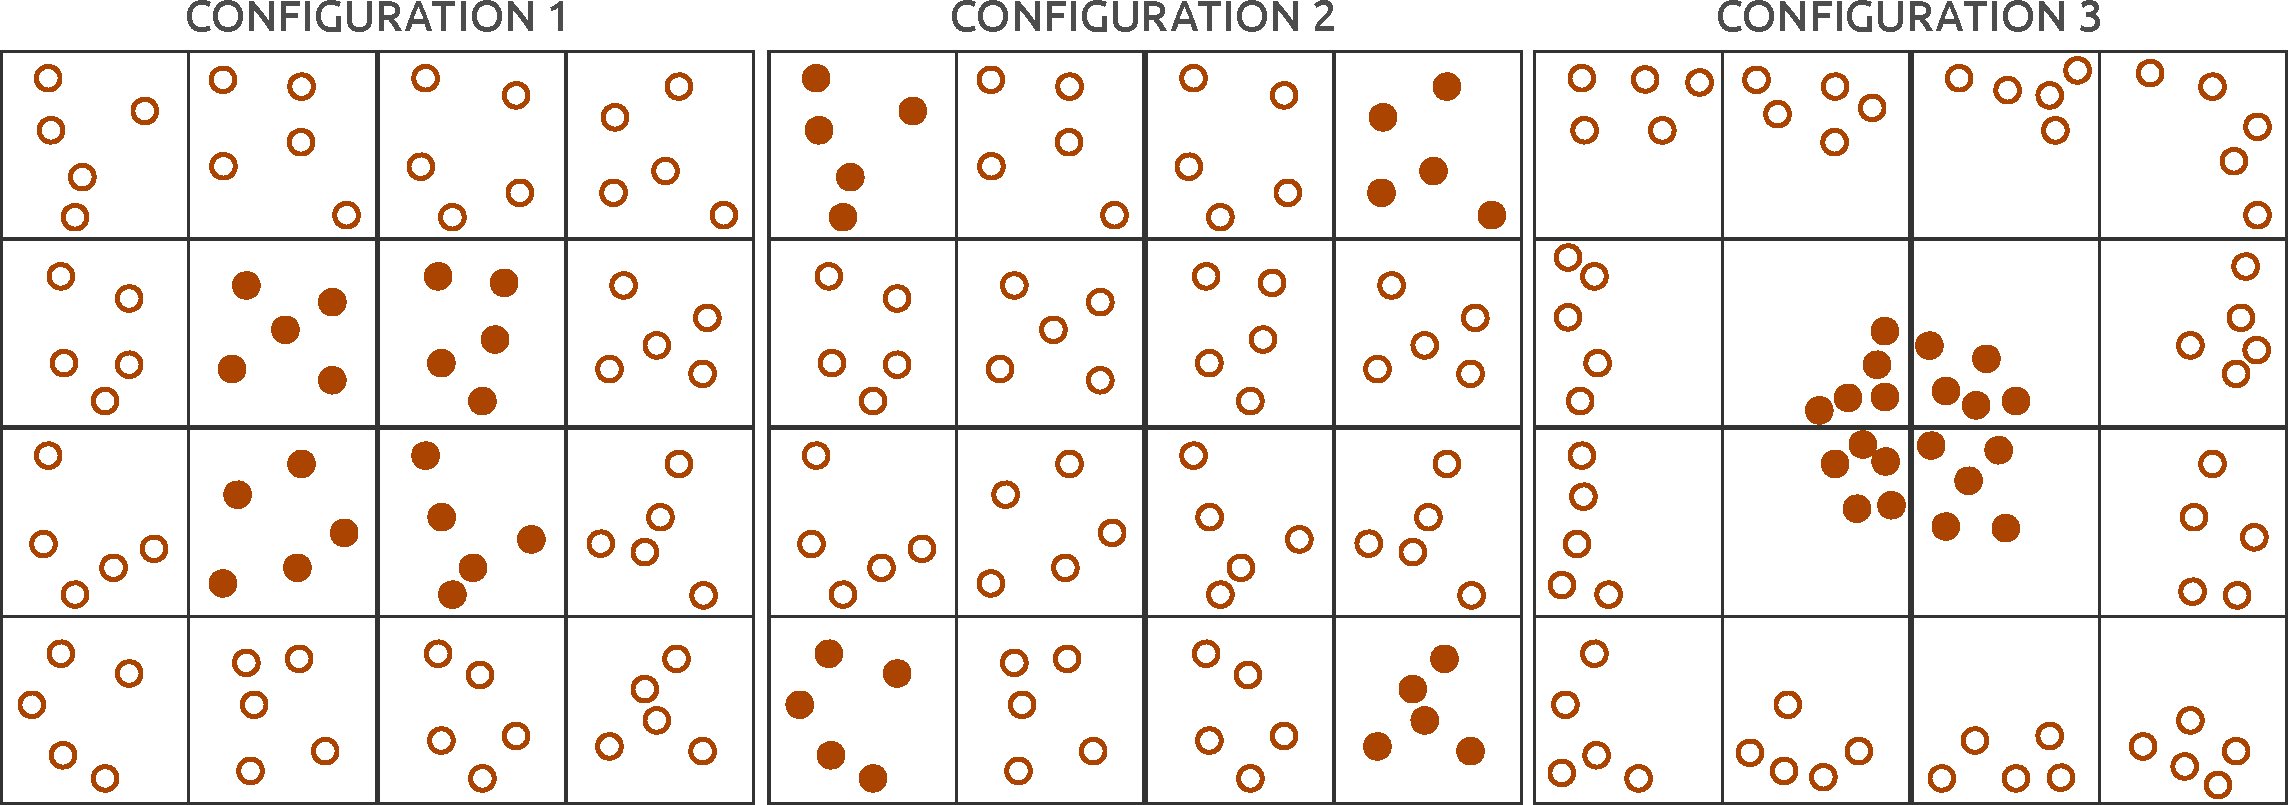
\includegraphics[width=12cm]{NonSpatial.pdf}
\end{figure}

Autocorrelation indexes (\textbf{Geary} and \textbf{Moran}) can distinguish between \textbf{1} et \textbf{2}.

\end{frame}


% FRAME
\begin{frame}{Autocorrelation}

Moran's I (1950):

$$
I = \frac{n}{\sum_{i} \sum_{j} w_{ij}} \times \frac{\sum_{i} \sum_{j} w_{ij} (x_i - \bar{x})(x_j - \bar{x})}{\sum_{i} (x_i - \bar{x})^2}
$$

~

$n$ : number of spatial units \\ 
$x_i$ et $x_j$ : values of $x$ in $i$ and $j$ \\ 
$\bar{x}$ : average value of $x$ \\ 
$w_{ij}$ : weighting matrix corresponding to the neighborhood definition

\end{frame}



% FRAME
\begin{frame}{Autocorrelation}

\textbf{Moran's I} interpretation based on \textbf{Moran's plot}

\begin{figure}
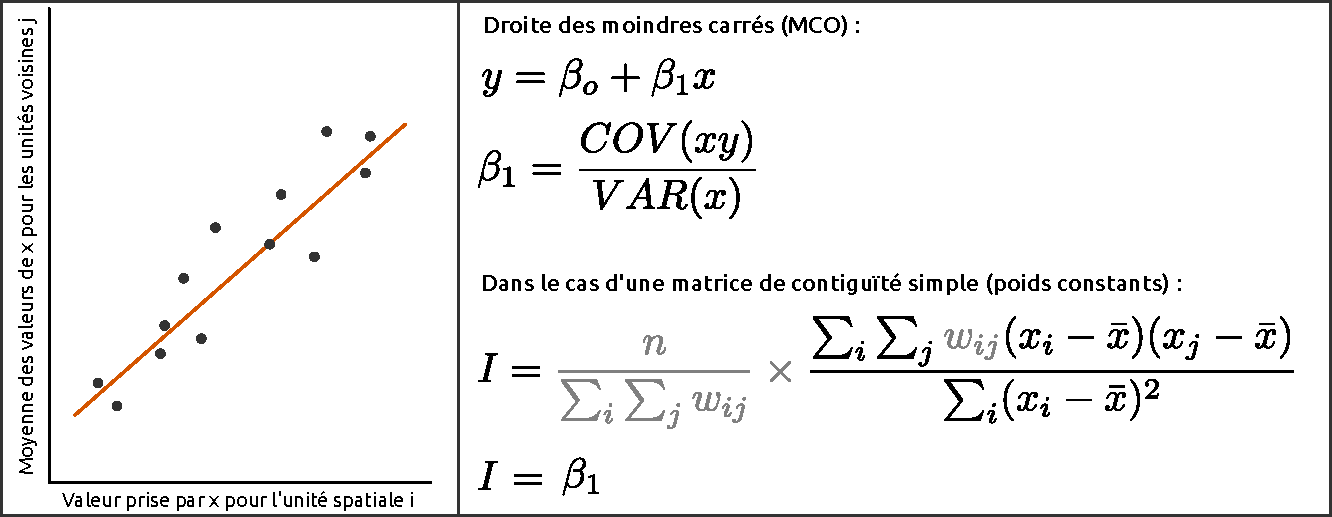
\includegraphics[width=12cm]{MoranPlot.pdf}
\end{figure}

\end{frame}


% FRAME
\begin{frame}{Autocorrelation}

\textbf{Local contribution to the global autocorrelation index} \\
LISA - \emph{local indicators of spatial autocorrelation}

$$
I_i = z_i \sum_{j} w_{ij} z_j
$$

~

$z_i$ standardized value of $x$ for spatial unit $i$ \\
$z_j$ standardized value of $x$ for spatial unit $j$ \\
$w_{ij}$ weighting matrix

\end{frame}


% FRAME
\begin{frame}{Spatial autoregressive model}

The autocorrelation can be used in a \textbf{descriptive} approach or in a \textbf{modeling} approach.

~

Ex. of land values modeling (econometrics): the value of a dwelling is function of:

\begin{itemize}
  \item Intrinsic attributes: surface area, garden, etc.
  \item Contextual attributes: i.e. the value of the dwellings in the neighborhood
\end{itemize}

~

In this case, it may be useful to build a \textbf{spatial autoregressive regression} (SAR), i.e. to inject the \textbf{lagged values} (neighborhood average) as a regressor.

\end{frame}

